\begin{titlepage}

\setlength{\hoffset}{-5mm}

\vspace*{-0.4cm}
%\begin{wrapfigure}{htb!l}{-0cm}
\begin{picture}(0,0)
    \put(-20,-40){
\includegraphics[width=340pt]{logos/Faculty_physics_goe}}%
\put(335,-41){
\includegraphics[width=95pt]{logos/Max-Planck-Gesellschaft}}\\
\end{picture}
%\end{wrapfigure}

\vspace*{0.27cm}
%\vspace*{-10pt}
\begin{flushright}
\rule{260pt}{0.4pt}\hspace{58pt}\space\space\space\space\space\space\space\space\space

\textsc{Fakult\"at f\"ur Physik \hspace{194pt}\space\space\space\space\space\space\space \\[5pt]}
\end{flushright}
\centering
\vspace*{2.cm}

%\textsc{\Large Bachelor's thesis}\\[6pt]
\textsc{\Large Specialization Report}\\[6pt]

%% fun only
%\textsc{\Large Specialization report}\\
%\textsc{\Small Iteration 2}\\
%% /fun only

\rule{400pt}{0.9pt}%\phantom{..}\\[15pt]
%\rule{400pt}{0.9pt}\\[0.5cm]
\textbf{\huge \vspace{5pt} \titel \vspace{5pt} \\[6pt] }
\rule{400pt}{0.9pt}\\[6pt]
\textbf{\large }

\vspace*{1.cm}
\textbf{\large Luis Miguel Ramos Henriques}\\[6pt]
 \texttt{l.ramoshenriques@stud.uni-goettingen.de}\\[32pt]

%\normalsize
\fontsize{10pt}{10pt}\selectfont

\begin{center}
%\begin{}
\begin{tabular}{rl}
%\text Author: &  \[6pt]
%Advisor \& First Referee: & \textbf{Dr. Marco G. Mazza}\\[2pt]
%Second Referee: & \textbf{Prof. Dr. Jörg Enderlein}\\
Advisor & \textbf{Dr. Marco G. Mazza}\\[2pt]

\end{tabular}
%\end{}
\end{center}

\vspace*{1.cm}
{26th June 2018}\\

\vspace*{1.5cm}

\textbf{
\rule{440pt}{1pt}\phantom{..}\\%[15pt]
\begin{minipage}[thb!]{0.40\textwidth}%
Max Planck Institute for\\
Dynamics and Self-Organization
\end{minipage}%
\begin{minipage}[htb!]{0.42\textwidth}%
\begin{flushright}
Research Group\\
\mbox{Nonequilibrium soft matter}
\end{flushright}
\end{minipage}
}
%\begin{flushright}
\begin{minipage}[htb!]{0.12\textwidth}%
~~~\includegraphics[width=70pt]{logos/logonesm}
\end{minipage}
%\end{flushright}

\end{titlepage}

%\thispagestyle{empty}
%\quad
%\newpage
% \setcounter{page}{1}
% \pagenumbering{roman}
%\begin{abstract}
% XXX

%Foo test abstract


%\thispagestyle{empty}
%\end{abstract}
%\newpage
% \\
% %

\iffalse %this is for the real thing
\newpage
\thispagestyle{empty}
\quad
\newpage
\setcounter{page}{1}
\pagenumbering{roman}

\tableofcontents

\newpage
\thispagestyle{empty}
\quad
\newpage
\fi
\tableofcontents
